
{ \small
% \vspace{-0.2cm}
\begin{figure}
\centering
\captionsetup{justification=centering}
\begin{subfigure}{.3\textwidth}
\begin{centering}
{\small
$
\begin{array}{l}
  \kw{nestedOdd}(n, m) \triangleq \\
  \clabel{ \assign{i}{n} }^{0} ; \\
      L_1: \ewhile ~ \clabel{i > 0}^{1} ~ \edo ~ \\
      \quad \big(
        \eif(\clabel{i \% 2 \neq 0 }^{2},\\
        \qquad \clabel{\assign{k}{i - m}}^{3};\\
        \qquad L_4: \ewhile ~ \clabel{k > 0}^{4} \edo \\
        \qquad \quad ( \clabel{\assign{k}{k - 1}}^{5} );\\
        \qquad \clabel{\assign{i}{k + m}}^{6};\\
        \qquad \clabel{\assign{i}{i - 1}}^{7}, \\
        \qquad \clabel{\assign{i}{i - 3}}^{8})
        \big)
  \end{array}
$
}
\caption{}
\end{centering}
\end{subfigure}
\begin{subfigure}{.35\textwidth}
\begin{centering}
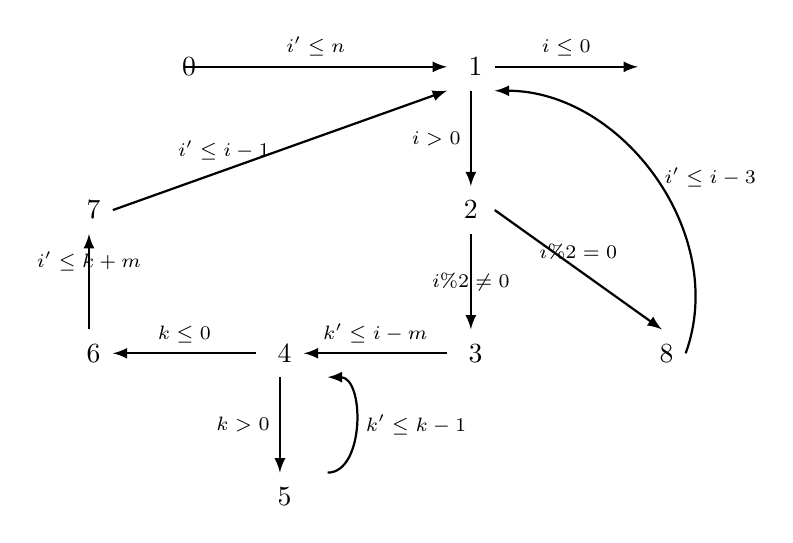
\begin{tikzpicture}[scale=\textwidth/20cm,samples=200]
\draw[] (-6, 10) circle (0pt) node{{ $0$}};
\draw[] (0, 10) circle (0pt) node{{ $1$}};
\draw[] (0, 7) circle (0pt) node{\textbf{$2$}};
\draw[] (0, 4) circle (0pt) node{{ $3$}};
\draw[] (-4, 4) circle (0pt) node{{ $4$}};
\draw[] (-8, 4) circle (0pt) node{{ $6$}};
\draw[] (-4, 1) circle (0pt) node{{ $5$}};
\draw[] (4, 4) circle (0pt) node{{ $8$}};
\draw[] (-8, 7) circle (0pt) node{{ $7$}};
% Counter Variables
\draw[] (4.5, 10) circle (0pt) node {\textbf{$\lex$}};
% \draw[] (6, 4) circle (0pt) node {{ $ex$}};
%
% Control Flow Edges:
\draw[ thick, -latex] (-6, 10)    -- node [above]{\scriptsize $i' \leq n$}(-0.5, 10);
\draw[ thick, -latex] (0, 9.5)    -- node [left] {\scriptsize $i > 0$} (0, 7.5) ;
\draw[ thick, -latex] (0.5, 7)    -- node [above] {\scriptsize $ i \% 2 = 0 $}  (4, 4.5);
\draw[ thick, -latex] (4.5, 4)    to  [out=70,in=0]   node [right] {\scriptsize $i' \leq i - 3$ }(0.5, 9.5);
\draw[ thick, -latex]  (0, 6.5)   -- node  {\scriptsize $i \% 2 \neq 0$}  (0, 4.5) ;
\draw[ thick, -latex]  (-0.5, 4)  -- node [above] {\scriptsize $k' \leq i - m$ }  (-3.5, 4) ;
\draw[ thick, -latex]  (-4.5, 4)  -- node [above] {\scriptsize $k \leq 0$ }  (-7.5, 4);
\draw[ thick, -latex] (0.5, 10)   -- node [above] {\scriptsize $i \leq 0$}  (3.5, 10);
\draw[ thick, -latex] (-4, 3.5)   -- node [left] {\scriptsize $k > 0$}  (-4, 1.5);
\draw[ thick, -latex] (-3, 1.5)   to  [out=0,in=0] node [right] {\scriptsize $k' \leq k- 1$}  (-3, 3.5);
\draw[ thick, -latex] (-8, 4.5)   --  node [above] {\scriptsize $i' \leq k + m$ }(-8, 6.5);
\draw[ thick, -latex] (-7.5, 7)  --  node [left] {\scriptsize $i' \leq i - 1$ }(-0.5, 9.5);
% \draw[ thick, -latex] (6, 6.5)  -- node [right] {$\top$} (6, 4.5) ;
\end{tikzpicture}
\caption{}
\end{centering}
\end{subfigure}
\begin{subfigure}{.3\textwidth}    
% \begin{centering}
{\small
$\tpath_0 = (0 \to 1)$
\\
$\tpath_1 = (1 \to 2 \to 3 \to 4)$
\\
$\tpath_2 = (4 \to 6 \to 7 \to 1)$
\\
$\tpath_3 = (4 \to 5 \to 4)$
\\
$\tpath_4 = (1 \to 2 \to 8 \to 1)$
\\
$\tpath_5 = (1 \to \lex)$
}
\caption{}
% \end{centering}
\end{subfigure}
% \vspace{-0.5cm}
\begin{subfigure}{.8\textwidth}    
  \begin{centering}
  $
  \tpath_0 ; \rpchoose{ 1: \rprepeat(\tpath_1; 4:\rprepeat(\tpath_3); \tpath_2; \tpath_4), 
  1: \rprepeat(\tpath_4; \tpath_1; 4:\rprepeat(\tpath_3); \tpath_2) }; \tpath_5
  $
  % \vspace{-0.5cm}
  \caption{}
  \end{centering}
  \end{subfigure}
\caption{
(a) Running example: program with a loop with two  paths and a nested loop in one of them,
(b) the corresponding \emph{abstract transition graph}, $\absG(\kw{nestedOdd}(n, m))$,
(c) all the simple transition paths on this program,
(d) the refined program.}
% \vspace{-0.75cm}      
\label{fig:relatedNestedWhileOdd-overview}
\end{figure}
}
%  \footnotetext{In the transition path, $(l_0 \to \cdots \to l_n)$, the constraints are omitted for concise.}
%
%  \end{example}    
